\documentclass[12pt,a4paper]{article}

% ----------------------
% Packages
% ----------------------
\usepackage[margin=2.5cm]{geometry}
\usepackage[utf8]{inputenc}
\usepackage[T1]{fontenc}
\usepackage{graphicx}
\usepackage{float}
\usepackage{amsmath}
\usepackage{xcolor}
\usepackage{listings}
\usepackage{hyperref}
\usepackage{enumitem}
\usepackage{booktabs}
\usepackage{longtable}
\usepackage{tikz}
\usepackage{titlesec}
\usepackage{parskip}
\usepackage{seqsplit}
\usetikzlibrary{arrows.meta, positioning, calc}

% ----------------------
% Colours
% ----------------------
\definecolor{codebg}{RGB}{245,245,245}
\definecolor{codekeyword}{RGB}{0,90,160}
\definecolor{codecomment}{RGB}{110,110,110}
\definecolor{codestring}{RGB}{160,40,40}
\definecolor{speedcolor}{RGB}{210,235,255}
\definecolor{batchcolor}{RGB}{255,230,200}
\definecolor{storecolor}{RGB}{225,245,225}
\definecolor{servecolor}{RGB}{240,225,250}

\lstdefinestyle{fleetiq}{
  backgroundcolor=\color{codebg},
  basicstyle=\ttfamily\small,
  keywordstyle=\color{codekeyword}\bfseries,
  commentstyle=\color{codecomment},
  stringstyle=\color{codestring},
  breaklines=true,
  breakatwhitespace=false,
  showstringspaces=false,
  frame=single,
  rulecolor=\color{gray!40},
  xleftmargin=1em,
  xrightmargin=0.5em,
  framexleftmargin=0.8em,
}
\lstset{style=fleetiq}

\titleformat{\section}{\Large\bfseries}{\thesection}{0.6em}{}
\titleformat{\subsection}{\large\bfseries}{\thesubsection}{0.6em}{}

\hypersetup{
  colorlinks=true,
  linkcolor=blue!55!black,
  citecolor=blue!55!black,
  urlcolor=blue!55!black,
  pdftitle={FleetIQ Project Report},
  pdfauthor={Dinidu Lochana},
}

\newcommand{\code}[1]{\texttt{#1}}
\newcommand{\tcode}[1]{\texttt{\seqsplit{#1}}}

% A simple dashed placeholder box for a screenshot that has not been
% pasted in yet. Replace with \includegraphics[width=...]{screenshots/...}
% once you have taken the real screenshot.
\newcommand{\screenshotbox}[3]{%
\begin{figure}[h]
\centering
\begin{tikzpicture}
\draw[dashed, thick, gray!70] (0,0) rectangle (#1,#2);
\node[align=center, text width=#1 cm - 1.5cm, gray!60] at ($(0,0)!0.5!(#1,#2)$)
  {[ Screenshot goes here ]\\[4pt]#3};
\end{tikzpicture}
\caption{#3}
\end{figure}
}

% ==================================================================
\begin{document}

% --- First Page (Cover Page) ---
\begin{titlepage}
    \centering
    \IfFileExists{Logo.jpeg}{%
        
\includegraphics[width=3cm]{Logo.jpeg}\par\vspace{1cm}
    }{%
        \par\vspace{0.3cm}{\small [Add Logo.jpeg to the report/ folder for the university logo]}\par\vspace{1cm}
    }
    {\LARGE \textbf{Department of Electrical and Information Engineering}}\\[0.4cm]
    {\Large \textbf{University of Ruhuna}}\\[1.5cm]
    {\Large \textbf{Mini Project Assessment}}\\[0.2cm]
    {\large \textbf{Big Data Analytics}}\\[0.2cm]
    {\large \textbf{EC8202}}\\[1.5cm]

   % Centered student and project info
    {\large \textbf{A Lambda Architecture Data Pipeline for Ride-Hailing Fleet Operations}}\\[0.8cm]
    {\large \textbf{Bandara M.M.D.L. - EG/2021/4434}}\\[0.4cm]
    {\large \textbf{Fernando K.M.K.N.C. - EG/2021/4508}}\\[0.4cm]
    {\large \textbf{Wijesinghe D.M.A.B. - EG/2021/4875}}\\[2cm]
    {\large \textbf{30/09/2026}}\\[2cm]



    \vfill
    Department of Electrical and Information Engineering\\
    University of Ruhuna\\[0.5cm]
    \vfill

\end{titlepage}

% ==================================================================
\section{Introduction}
% ==================================================================

Ride-hailing companies run many vehicles at once. Two different kinds of
information matter to them. First, they need to know what their vehicles are
doing right now: which cars are busy, which are sitting idle, and how
much money is being earned in each part of the city. Second, once a day, they
need to know the real cost of running each vehicle, because garages
and fuel stations send their bills once a day, not every second.

FleetIQ is a small but complete system that answers both needs. It listens to
a stream of GPS events from a simulated fleet of vehicles, and it also reads
a daily file of vehicle expenses. It cleans, joins, and summarises this data,
then shows the results on a live dashboard and through a set of report
pages. The system also watches itself, so that if something stops working,
an alert is raised automatically instead of a person having to notice by
chance.

\subsection{Use Case}

The chosen use case is \textbf{Ride-Hailing Fleet Operations}. A ride-hailing
operator wants to see, in real time, how well its fleet is being used. At
the same time, it wants a daily check of which vehicles are actually
profitable once fuel and maintenance costs are taken into account.

\begin{itemize}
  \item \textbf{Streaming source:} A GPS/telemetry event for every trip,
    sent every few seconds. Each event has a trip ID, driver ID, vehicle ID,
    location (latitude and longitude), speed, status (idle, enroute, or
    on\_trip), and fare earned so far.
  \item \textbf{Daily-batch source:} One file per day, listing each
    vehicle's fuel cost, maintenance cost, distance driven, and whether it
    needed a service that day. This file comes from garages and fuel
    partners, and it only arrives once a day.
\end{itemize}

\subsection{Business Requirements}

Reading the use case carefully, the following requirements can be pulled
out. These requirements shaped every design choice made later in this
report.

\begin{enumerate}
  \item The system must show, at any moment, how many vehicles are active,
    how many are idle, and how much money is being earned, broken down by
    area of the city.
  \item The system must combine the day's driving activity with the day's
    real costs, and work out which vehicles made a profit and which did not.
  \item The system must not lose or block the live view while it waits for
    the daily cost file. The two jobs must be able to run independently.
  \item The system must tell someone, without being asked, when something is
    wrong - for example, no GPS data arriving, or a vehicle sitting idle
    for too long.
  \item All of this must be visible through one simple place: a dashboard
    and a small set of report pages, backed by a real, queryable database.
\end{enumerate}

% ==================================================================
\section{Architecture Decision: Lambda vs.\ Kappa}
% ==================================================================

Before writing any code, a choice had to be made between two well-known
ways of building a big data pipeline: \textbf{Lambda architecture} and
\textbf{Kappa architecture}. This section explains both in simple terms,
then explains why Lambda was chosen and why Kappa was rejected.

\subsection{What Lambda Architecture Means}

A Lambda architecture uses \textbf{two separate paths} to handle data:

\begin{itemize}
  \item A \textbf{speed layer} that processes data as it arrives, giving
    fast but "best effort" results. If one GPS point is a little late or
    slightly wrong, it does not matter much, because the next update will
    correct the picture a few seconds later.
  \item A \textbf{batch layer} that runs on a schedule (for example, once a
    day) and works out the correct, final answer from a complete set of
    data. If a mistake is found later, this layer can simply be run again
    for that one day, without touching anything else.
\end{itemize}

Both layers write their results into the same storage, which a single
serving layer (an API and a dashboard) reads from. The speed layer gives
users something to look at immediately; the batch layer is the layer that
is trusted to be correct.

\subsection{What Kappa Architecture Means}

A Kappa architecture is simpler in structure: there is only \textbf{one}
path. Every kind of data, including data that would normally be a "batch"
file, is treated as an event stream. If something needs to be corrected or
recomputed, the fix is to replay the stream through an updated version of
the same processing job. There is no separate batch system.

\subsection{Why FleetIQ Uses Lambda}

The two FleetIQ data sources behave very differently, and this difference
is exactly what Lambda architecture is designed for.

\begin{itemize}
  \item \textbf{GPS telemetry} needs to feel live. It arrives every few
    seconds, and small errors do not matter, because the vehicle sends a new
    position moments later anyway. This is a natural fit for a speed layer.
  \item \textbf{Vehicle expenses} need to be correct, not fast. They arrive
    once a day from an outside partner. If a garage sends a wrong invoice
    and later sends a corrected one, the fix should simply be: run that
    one day's cost calculation again. This must happen without
    touching or restarting the live GPS pipeline, because the two problems
    are completely independent.
\end{itemize}

Because the two sources have different jobs to do - one must be fast, the
other must be correct and easy to redo - keeping them as two separate
pipelines that both feed the same storage is the natural choice. This is
precisely the Lambda pattern.

\subsection{Why Kappa Was Rejected}

Kappa architecture was considered and rejected for this project, for a
specific reason: Kappa works best when the "batch" data is really just
old stream data being replayed. In FleetIQ, that is not true. The
daily expense file is not a recording of an earlier stream - it is a
genuinely separate, once-a-day feed sent by an outside company. Forcing it
through the same continuous stream-processing engine as the live GPS data
would not add any benefit. It would only make the system more complicated,
because now the "fix yesterday's invoice" problem and the "track live GPS"
problem would be tangled together inside one engine, when in reality they
have nothing to do with each other. For this reason, Lambda architecture,
with its clean separation between the speed layer and the batch layer, was
the better and simpler choice for FleetIQ.

% ==================================================================
\section{System Architecture}
% ==================================================================

Figure~\ref{fig:architecture} shows the overall design of FleetIQ, split
into the four layers asked for in the brief: ingestion, processing,
storage, and serving.

\begin{center}
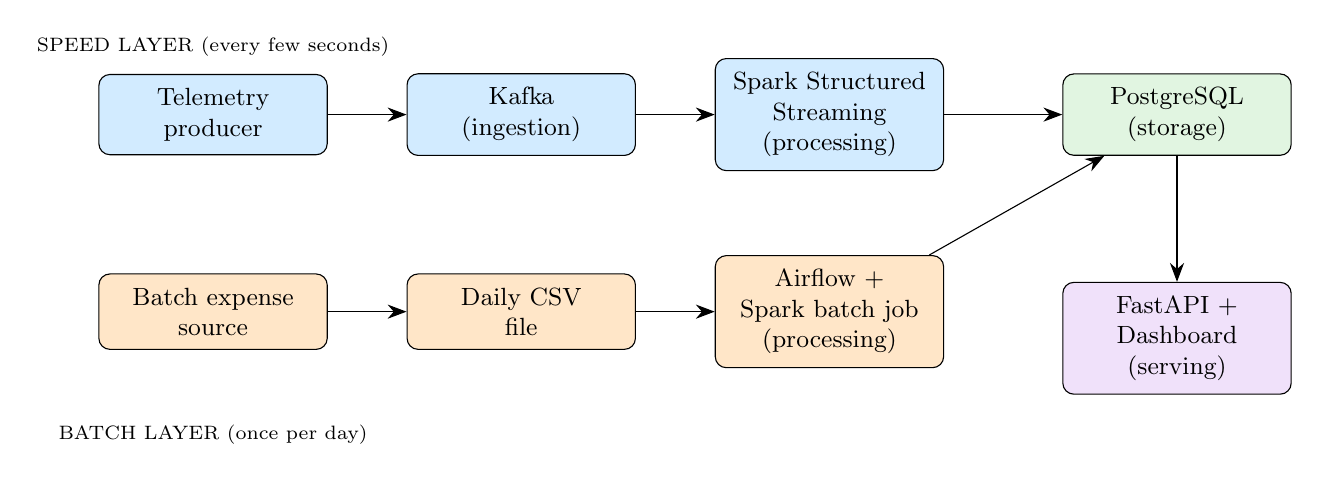
\begin{tikzpicture}[
    box/.style={draw, rounded corners, minimum width=2.9cm, minimum height=0.9cm, align=center, font=\small, inner sep=5pt},
    lbl/.style={font=\scriptsize, align=center},
    >={Stealth[length=2.4mm]}, node distance=0.9cm and 1.0cm
  ]
  \node[box, fill=speedcolor] (producer) {Telemetry\\producer};
  \node[box, fill=speedcolor, right=of producer] (kafka) {Kafka\\(ingestion)};
  \node[box, fill=speedcolor, right=of kafka] (spark) {Spark Structured\\Streaming\\(processing)};
  \node[box, fill=storecolor, right=1.5cm of spark] (pg) {PostgreSQL\\(storage)};

  \draw[->] (producer) -- (kafka);
  \draw[->] (kafka) -- (spark);
  \draw[->] (spark) -- (pg);

  \node[box, fill=batchcolor, below=1.5cm of producer] (batchsrc) {Batch expense\\source};
  \node[box, fill=batchcolor, right=of batchsrc] (landing) {Daily CSV\\file};
  \node[box, fill=batchcolor, right=of landing] (airflow) {Airflow +\\Spark batch job\\(processing)};

  \draw[->] (batchsrc) -- (landing);
  \draw[->] (landing) -- (airflow);
  \draw[->] (airflow) -- (pg);

  \node[box, fill=servecolor, below=1.6cm of pg] (api) {FastAPI +\\Dashboard\\(serving)};
  \draw[->] (pg) -- (api);

  \node[lbl, above=0.1cm of producer] {SPEED LAYER (every few seconds)};
  \node[lbl, above=0.1cm of batchsrc, yshift=-2.4cm] {BATCH LAYER (once per day)};
\end{tikzpicture}
\end{center}
\begin{center}
\refstepcounter{figure}
\label{fig:architecture}
Figure \thefigure: FleetIQ system architecture, showing the four required layers.
\end{center}

\subsection{Ingestion Layer}
A Python script simulates a fleet of vehicles and sends one GPS event per
vehicle every few seconds to \textbf{Apache Kafka}. Kafka is a message
queue: it safely holds the incoming events so that the processing layer can
read them at its own pace, even if it falls behind for a moment.

\subsection{Processing Layer}
Two different processing jobs exist, matching the two layers of the Lambda
design:
\begin{itemize}
  \item The \textbf{speed layer} uses \textbf{Apache Spark Structured
    Streaming} to read from Kafka continuously. It cleans bad data,
    enriches each event with extra information (such as which city zone it
    happened in), and calculates rolling totals (such as earnings per zone
    per minute).
  \item The \textbf{batch layer} uses \textbf{Apache Airflow} to run a
    small \textbf{Spark} job once a day. This job joins the day's driving
    totals with the day's cost file, and works out which vehicles were
    profitable.
\end{itemize}

\subsection{Storage Layer}
All results are saved into a single \textbf{PostgreSQL} database, so both
layers write into one shared place. In addition, the daily batch job also
saves a copy of its results as \textbf{Parquet} files on disk. Parquet is a
compact file format that is good for storing historical records that can be
read again later, even outside the database.

\subsection{Serving Layer}
A small \textbf{FastAPI} web service reads from PostgreSQL and answers
requests for the live numbers, the daily report, and the current alerts. A
simple web dashboard, built with plain HTML and JavaScript, calls this API
every few seconds and shows the numbers on screen.

% ==================================================================
\section{Technology Stack and Justification}
% ==================================================================

Table~\ref{tab:stack} lists every major tool used in FleetIQ and explains,
in simple terms, why it was chosen for its job.

\begin{center}
\begin{longtable}{@{}p{2.6cm}p{3.4cm}p{8.2cm}@{}}
\caption{Technology stack and the reason each tool was chosen.}
\label{tab:stack}\\
\toprule
\textbf{Layer} & \textbf{Tool} & \textbf{Reason for choosing it} \\
\midrule
\endhead
Ingestion & Apache Kafka & Kafka can accept many small messages arriving
  quickly, from many vehicles at once, without losing them. It also keeps
  the producer (the vehicle) and the consumer (the processing job) separate,
  so one can be slow or restart without breaking the other. \\
Speed-layer processing & Spark Structured Streaming & Spark can read
  directly from Kafka and has built-in support for time windows (for
  example, "add up earnings for each 1-minute period"). This is exactly the
  kind of live summarising this project needs. \\
Batch orchestration & Apache Airflow & The daily job has clear steps that
  must happen in order: wait for the file, load it, run the calculation,
  then check the result. Airflow is built exactly for scheduling and
  running this kind of multi-step job, and it also retries automatically if
  a step fails. \\
Storage and serving & PostgreSQL & PostgreSQL lets the dashboard ask quick
  questions like "show me the last 10 minutes for this zone" using normal,
  well-understood database queries. \\
Extra batch storage & Parquet files & Parquet keeps a permanent, compact
  copy of each day's report on disk, separate from the live database. This
  is useful for keeping history safe even if the database is ever reset. \\
\bottomrule
\end{longtable}
\end{center}

Two alternatives named in the assignment brief were considered and not
used, for simple reasons:

\begin{itemize}
  \item \textbf{Apache Storm} was considered instead of Spark Structured
    Streaming. Storm processes one record at a time and is built for
    extremely low delay. FleetIQ does not need that level of speed - a
    delay of a few seconds is completely fine - so Spark's easier
    time-window tools were a better fit.
  \item \textbf{Cassandra} was considered instead of PostgreSQL. Cassandra
    is built for very large amounts of fast, simple writes spread across
    many machines. At the size of this project (a few dozen simulated
    vehicles), that scale is not needed, and PostgreSQL's ability to answer
    more complex questions easily made it the better choice.
\end{itemize}

% ==================================================================
\section{Observability Design}
% ==================================================================

A pipeline that no one can check is not trustworthy. FleetIQ was built with
three simple but effective ways to see what is happening inside it, and to
be told automatically when something goes wrong.

\subsection{What Is Measured}

\begin{itemize}
  \item \textbf{Logs from every stage.} Every part of the system - the
    two data sources, both processing jobs, the API, and the watchdog -
    writes log lines in the same simple format (one line of readable text
    per event, including a timestamp and which part of the system it came
    from).
  \item \textbf{Health of every part.} Each major part regularly writes
    "I am alive, and this is the last time I did useful work" into a small
    database table.
  \item \textbf{Basic metrics.} The API exposes simple counters and
    measurements, such as how many seconds have passed since the last GPS
    event arrived, in a standard format that monitoring tools can read.
\end{itemize}

\subsection{How It Is Measured}

A small background script, called the \textbf{watchdog}, wakes up every
30 seconds and checks the health information described above. If it finds a
problem, it writes an alert into an alerts table. The same alert is
automatically marked as resolved once the problem goes away, so old,
fixed problems do not keep cluttering the alert list.

\subsection{Why This Matters}

Without this, a manager would only find out about a broken pipeline by
noticing that the dashboard numbers had stopped changing - which could
take hours. With these checks running constantly, a problem is flagged
within seconds to minutes of it happening, which matches how a real
operations team would expect to be told about a fault.

\subsection{Alert Rules}

Three simple rules were implemented, matching the kind of alerts a real
fleet operator would actually want:

\begin{enumerate}
  \item \textbf{No GPS data for 60 seconds.} This means the live pipeline
    has stopped working. A \textbf{critical} alert is raised.
  \item \textbf{A vehicle idle for more than 2 minutes.} This means a
    vehicle is not being used, which wastes money. A \textbf{warning}
    alert is raised. This is the exact example given in the assignment
    brief.
  \item \textbf{The daily report is missing, or most of the fleet looks
    unprofitable.} This is checked as the last step of the daily batch job,
    and raises an alert if either case is true, since both would suggest
    something went wrong with that day's calculation.
\end{enumerate}

% ==================================================================
\section{Results: Sample Output}
% ==================================================================

This section shows real output taken from a running copy of FleetIQ, to
demonstrate that the whole pipeline actually works end to end, not just on
paper.

\subsection{Live Dashboard}

The dashboard is a single web page that updates itself every four seconds.
It shows the current number of active vehicles, the idle ratio, trips in
the last hour, a table of activity per city zone, a list of current
alerts, and a table for the daily profitability report.

\begin{figure}[H]
\centering
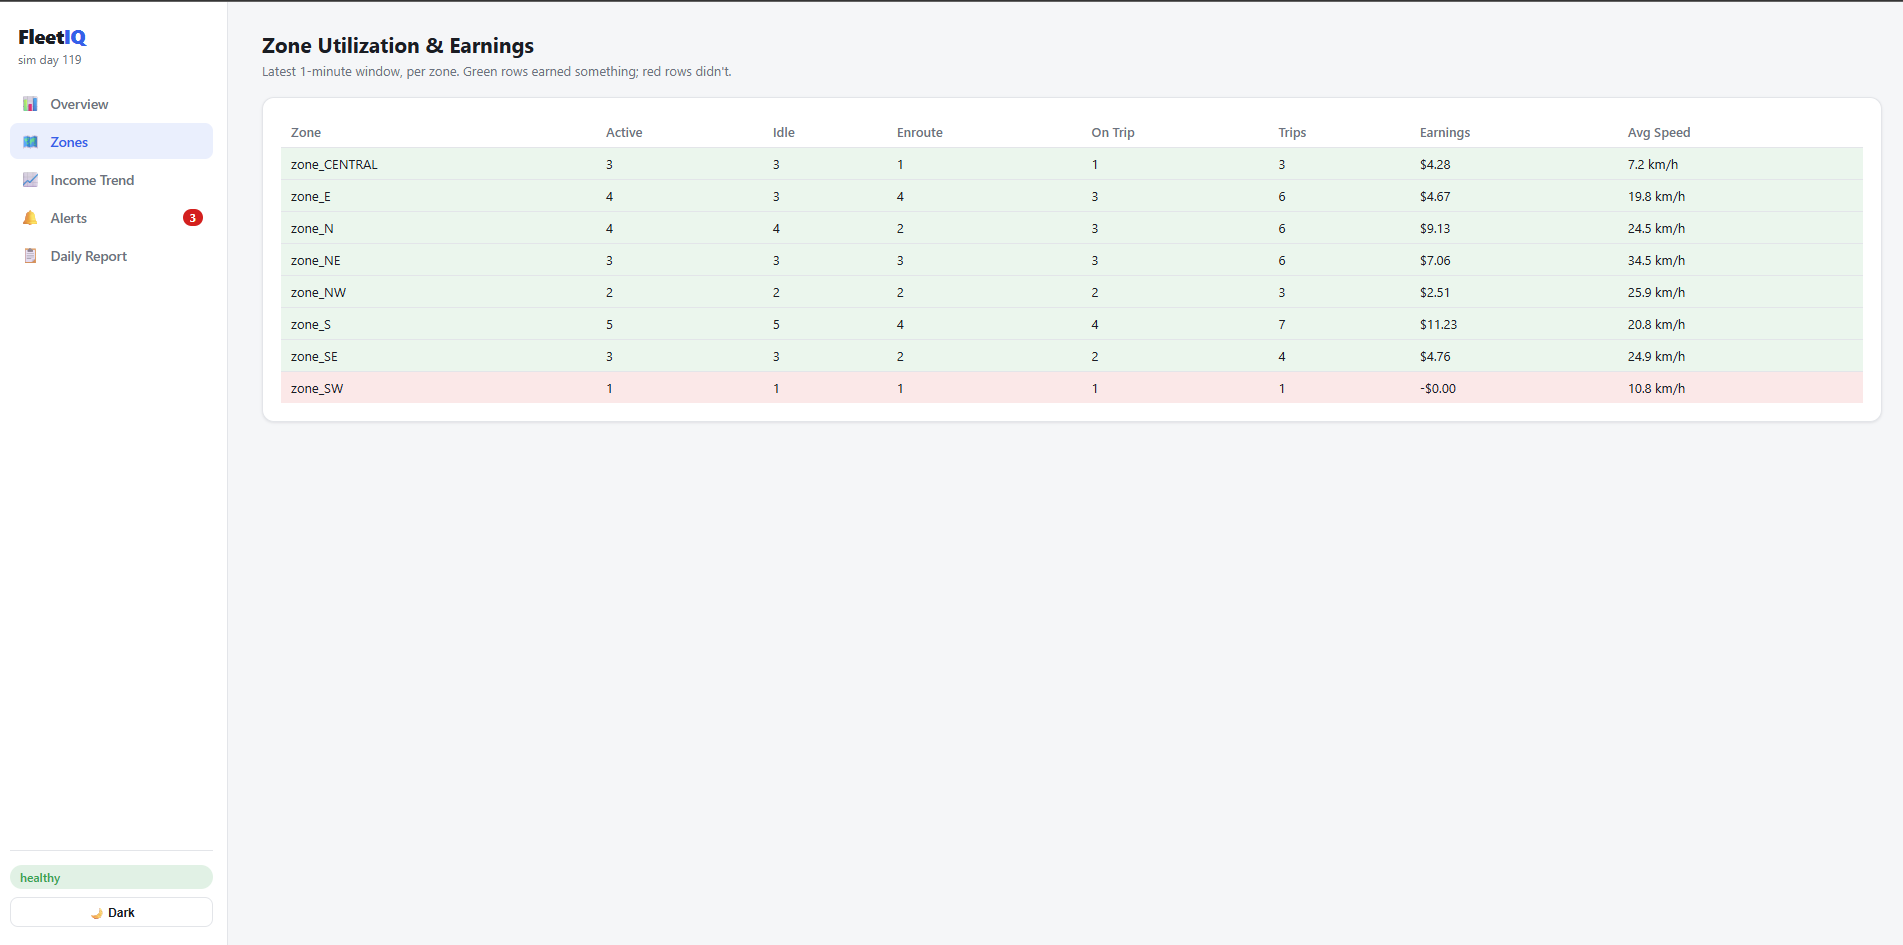
\includegraphics[width=\textwidth]{screenshots/dashboard.png}
\caption{The FleetIQ dashboard, showing live vehicle counts and zone activity.}
\end{figure}

\subsection{Sample API Output}

The API returns simple, readable JSON. Below is a real response captured
from the health check endpoint while the system was running normally.

\begin{lstlisting}[caption={A real response from \texttt{GET /health}}]
{
  "status": "healthy",
  "sim_day": 164,
  "telemetry_lag_seconds": 6.7,
  "staleness_threshold_seconds": 60,
  "components": [
    {"component": "stream-processor", "status": "healthy"},
    {"component": "watchdog",         "status": "healthy"},
    {"component": "airflow-reconciliation", "status": "healthy"}
  ]
}
\end{lstlisting}

A second real response, from the live-metrics endpoint, shows the kind of
answer the dashboard's zone table is built from:

\begin{lstlisting}[caption={A real response from \texttt{GET /metrics/realtime} (shortened)}]
{
  "sim_day": 164,
  "active_vehicles": 24,
  "idle_ratio": 0.375,
  "status_breakdown": {"idle": 9, "on_trip": 10, "enroute": 5},
  "trips_last_hour": 120,
  "zones": [
    {"zone": "zone_CENTRAL", "active_vehicles": 24,
     "trip_count": 35, "total_earnings": 37.49, "avg_speed": 21.3}
  ]
}
\end{lstlisting}

\subsection{Sample Daily Profitability Report}

Table~\ref{tab:profitability} shows real output from the daily batch
reconciliation job, for one simulated day. It shows the four most
unprofitable and four most profitable vehicles out of the full fleet of
24. This is exactly the answer the assignment's business question asks
for: which vehicles are becoming unprofitable once the day's real
costs are known.

\begin{center}
\begin{longtable}{@{}lrrrrp{3.6cm}@{}}
\caption{Sample profitability results for one simulated day (real captured output).}
\label{tab:profitability}\\
\toprule
\textbf{Vehicle} & \textbf{Fare (\$)} & \textbf{Fuel (\$)} & \textbf{Maint. (\$)} & \textbf{Net Profit (\$)} & \textbf{Result} \\
\midrule
\endhead
V018 & 3.42 & 0.19 & 45.86 & $-$42.64 & Unprofitable (repair spike) \\
V003 & 0.00 & 0.03 & 17.75 & $-$17.78 & Unprofitable (no trips, repair) \\
V024 & 0.00 & 0.00 & 4.12  & $-$4.12  & Unprofitable (idle all day) \\
V006 & 1.75 & 0.11 & 4.70  & $-$3.06  & Unprofitable \\
\midrule
V010 & 3.80 & 0.28 & 2.83  & 0.69     & Profitable \\
V009 & 3.43 & 0.16 & 2.44  & 0.83     & Profitable \\
V023 & 3.84 & 0.25 & 2.25  & 1.34     & Profitable \\
V022 & 5.07 & 0.27 & 2.32  & 2.48     & Profitable \\
\bottomrule
\end{longtable}
\end{center}

This table tells a clear, realistic story. Vehicle V018 looks fine day to
day, but a single large repair bill made it deeply unprofitable for that
day. Vehicle V024 never got any trips at all, so it earned nothing while
still costing money to keep on the road - exactly the kind of vehicle a
manager would want flagged. The best vehicles, like V022, simply completed
more paid trips than they spent on fuel and upkeep. This is a genuine,
useful business answer, not just raw numbers.

\subsection{Airflow Batch Run}

The daily reconciliation job is visible in the Airflow web interface as a
sequence of five steps: compute the day, wait for the file, load it, run
the calculation, then check the result. A successful run shows all five
steps in green.

\begin{figure}[H]
\centering
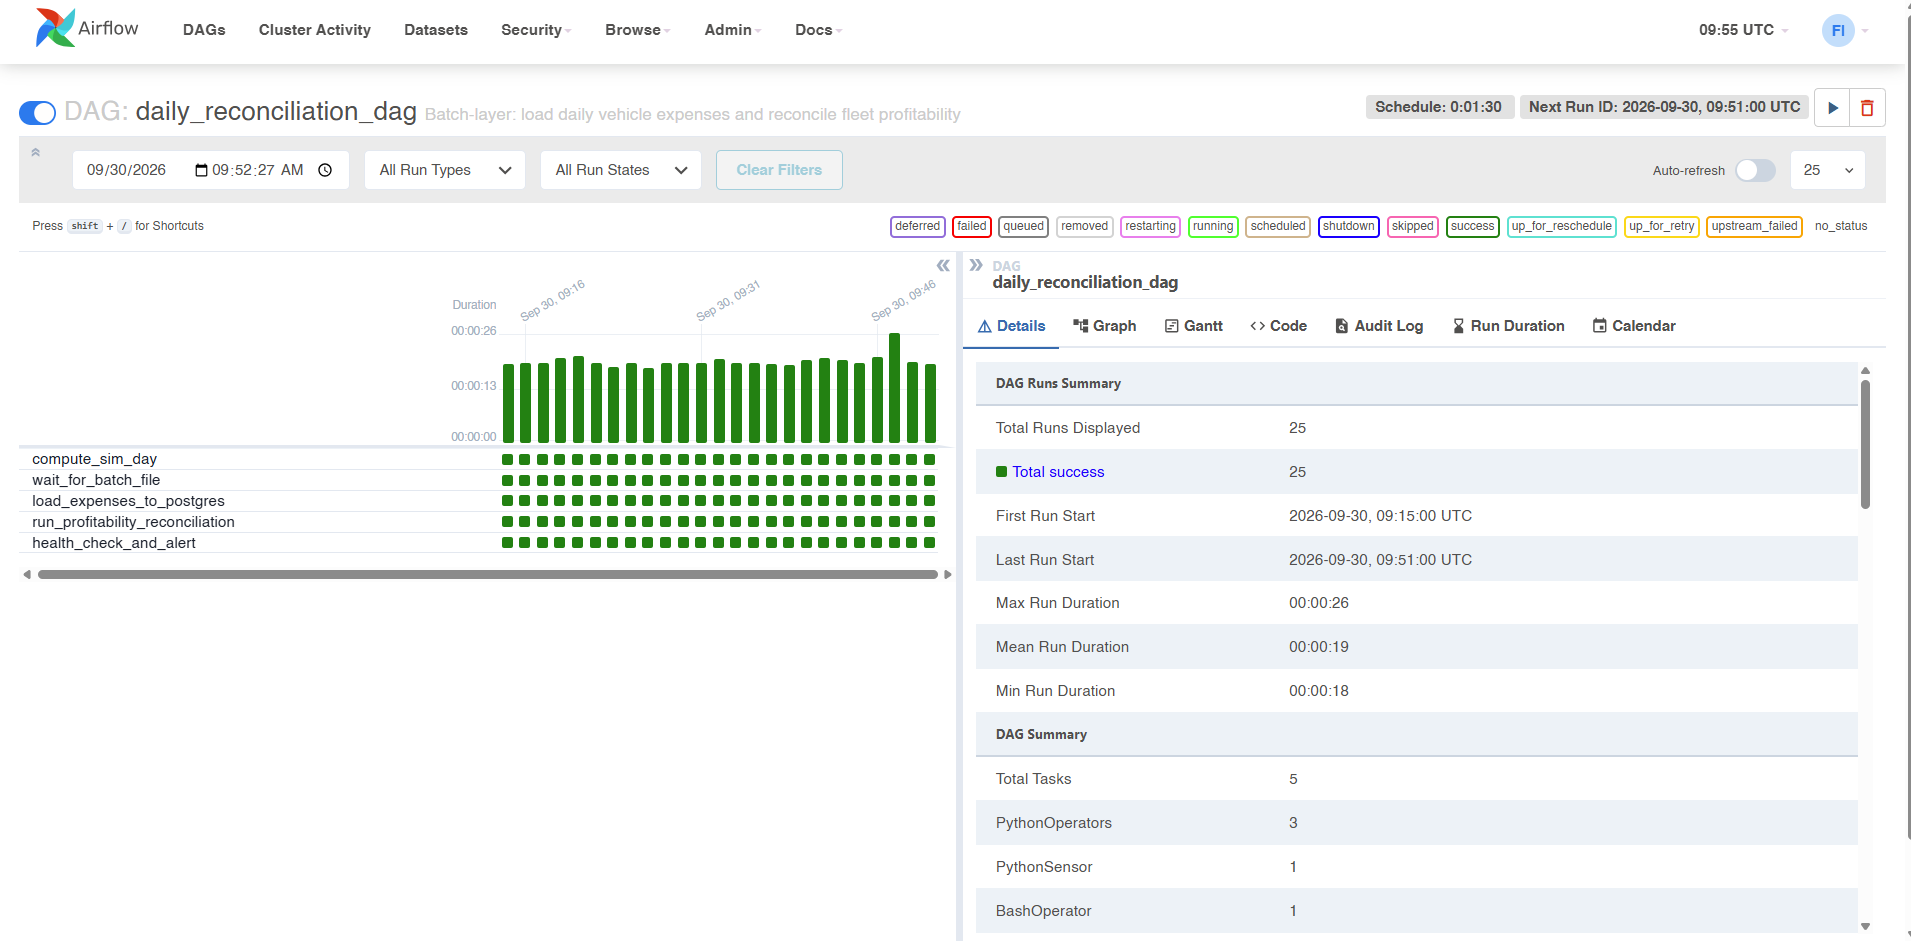
\includegraphics[width=\textwidth]{screenshots/airflow_dag.png}
\caption{A completed Airflow DAG run, showing all five reconciliation steps succeeded.}
\end{figure}

% ==================================================================
\section{Limitations, Trade-offs, and Production-Scale Improvements}
% ==================================================================

FleetIQ works well for its purpose: a class project demonstrating a full
Lambda pipeline on a laptop, with a simulated fleet of about two dozen
vehicles. Several choices were made to keep the system simple and reliable
at this small scale. This section lists those choices honestly, and
explains what would need to change for a real, much larger fleet.

\subsection{Current Limitations}

\begin{itemize}
  \item \textbf{Spark runs on one machine, not a cluster.} This keeps setup
    simple and avoids extra moving parts. It works fine for a few dozen
    vehicles, but a real fleet of thousands of vehicles would need Spark
    spread across several machines.
  \item \textbf{Saving results uses simple update-or-insert calls, not a
    dedicated streaming write tool.} Every table FleetIQ writes to needs to
    either add a new row or update an existing one, so each small batch of
    processed data is collected and written using ordinary database
    commands. This is simple and easy to understand, but it would become
    slow if the fleet size grew very large.
  \item \textbf{The running daily-earnings total is never automatically
    cleared out.} The system currently keeps every day's running total in
    memory for as long as it is running, without removing old, no-longer-needed
    days. For a short class demonstration, this is not a problem, but a
    system that runs for months would need a way to clear out very old data
    automatically.
  \item \textbf{The data is simulated, not real.} Real GPS devices would
    sometimes send duplicate messages, arrive late, or send incorrect
    readings in more varied and unpredictable ways than the simulation
    does. A production system would need extra checks to handle this
    messier reality.
  \item \textbf{Only three alert rules exist.} This satisfies the
    assignment's requirement, but a real operations team would likely want
    more - for example, alerts based on unusual patterns, not just fixed
    thresholds.
\end{itemize}

\subsection{What Would Change at Production Scale}

\begin{enumerate}
  \item \textbf{Move Spark to a real cluster.} Instead of running on one
    machine, the same Spark code would run across several worker machines,
    letting the system handle far more vehicles and far more events per
    second.
  \item \textbf{Use a proper streaming write tool.} Instead of collecting
    small batches and writing them with ordinary database commands, a tool
    such as Kafka Connect, or a change-data-capture tool, would be used to
    write results into the database continuously and more efficiently.
  \item \textbf{Split storage by purpose.} The huge, fast-growing table of
    raw GPS events would likely move to a database built for large-scale
    writes, such as Cassandra, while PostgreSQL would be kept only for the
    smaller, already-summarised tables the dashboard reads from. This
    matches the "Cassandra for very high write-throughput telemetry"
    option mentioned in the assignment brief.
  \item \textbf{Add real alerting and dashboards.} A production system
    would connect its metrics to a proper monitoring dashboard (such as
    Grafana) and send alerts to a paging system, so that on-call staff are
    contacted directly instead of only seeing alerts inside the app.
  \item \textbf{Handle messier real-world data.} Extra logic would be added
    to detect and safely ignore duplicate GPS messages, handle clock
    differences between devices, and deal with late or missing daily cost
    files without stopping the whole pipeline.
\end{enumerate}

% ==================================================================
\section{Conclusion}
% ==================================================================

FleetIQ shows a complete, working example of a Lambda architecture data
pipeline, built specifically around the needs of a ride-hailing fleet
operator. The business question - what is happening right now, and which
vehicles are losing money once real costs are known - is answered by
splitting the work into a fast speed layer and a correct, re-runnable batch
layer, exactly as Lambda architecture recommends. The
system also watches its own health and raises alerts automatically,
meeting the observability requirement. The results shown in this report,
including a real profitability table, prove that the pipeline produces a
genuinely useful answer to the business question it was built to solve.

\end{document}
